%\section{Introducción}

El presente documento describe el desarrollo de un m\'{e}todo para la detecci\'{o}n de anomal\'{i}as en la conducci\'{o}n. Se propone el uso de t\'{e}cnicas de Inteligencia Artificial para generar un mecanismo que identifique anomal\'{i}as de manejo, de tal modo que \'{e}stas puedan usarse para alertar oportunamente a los agentes y as\'{i} logren correjir sus conductas de manejo.

\vspace{5mm} %5mm vertical space

La idea principal, es generar un modelo que aprenda el comportamiento normal de conducci\'{o}n de un usuario concreto, para posteriormente detectar de forma aut\'{o}noma aquellos comportamientos inesperados e informarlos como anomal\'{i}as, de manera que se pueda evitar  un accidente de tr\'{a}nsito o reducir los efectos del mismo.

\section{Planteamiento del problema}

Debido a las graves secuelas que causan sobre las personas y los altos costos econ\'{o}micos asociados a ellos, los accidentes de tr\'{a}nsito se catalogan como un problema social y de salud p\'{u}blica mundial.

\vspace{5mm} %5mm vertical space

Seg\'{u}n la Organizaci\'{o}n Mundial de Salud (OMS) cada a\~{n}o existen aproximadamente 1,25 millones de muertes a causa de accidentes de tr\'{a}nsito, agregando que la mitad de todas estas victimas son peatones, ciclistas y motociclistas (V\'{e}ase la figura \ref{fig:oms} pag. \pageref{fig:oms}). Asimismo se puede decir que son una de las causas de muerte más importantes en el mundo, y la principal causa de muerte entre personas de edades comprendidas entre los 15 y los 29 años. 

\vspace{5mm} %5mm vertical space

\begin{figure}[h!]
  \begin{center}	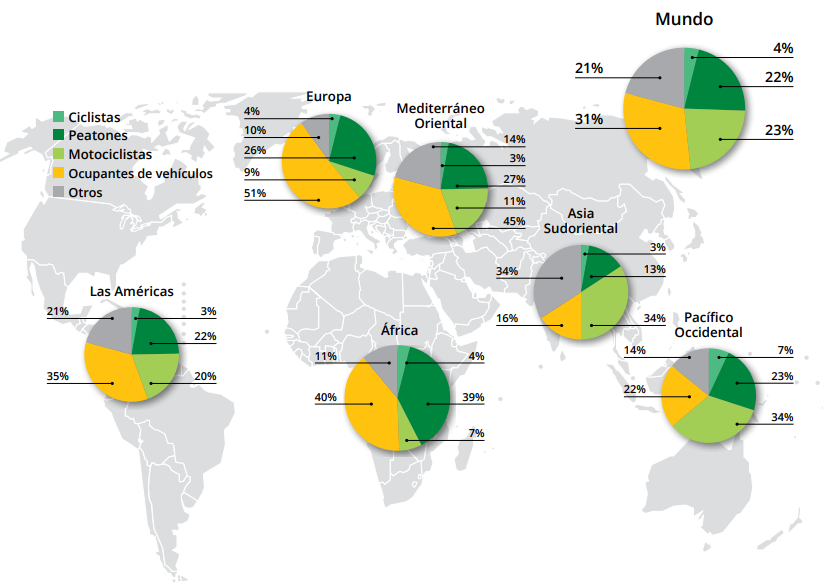
\includegraphics[width=0.9\textwidth]{imagenes/Cap1/oms1}
  \caption{Muertes por accidentes de tránsito por regi\'{o}n en función del tipo de usuario (2013), OMS}
  \label{fig:oms}  
  \end{center}
\end{figure}

Por otro lado seg\'{u}n la Unidad Operativa de Tr\'{a}nsito de Cochabamba los accidentes registrados en 2017 provocaron la muerte de 200 personas y dejaron aproximadamente 2200 heridos.
	
\vspace{5mm} %5mm vertical space

En la figura \ref{fig:arbol} se muestra las causas por las cuales se ocasiona un accidente de tr\'{a}nsito, se puede observar que gran parte de \'{e}stas se deben al factor humano sin embargo hay otras que conllevan factores medio-ambientales y mec\'{a}nicos, por lo que se hace imposible evitar completamente los mismos. 

\vspace{5mm} %5mm vertical space

Es por ello que se hace necesario el contar con mecanismos para prevenir y/o actuar de forma oportuna ante posibles accidentes de tr\'{a}nsito, motivo por el cual el presente trabajo se centra en estudiar los comportamientos de conducci\'{o}n, para as\'{i} generar alertas al encontrar un comportamiento an\'{o}malo en el manejo, de manera que se pueda evitar o en todo caso minimizar los efectos del mismo.

\begin{figure}[h!]
  \begin{center}	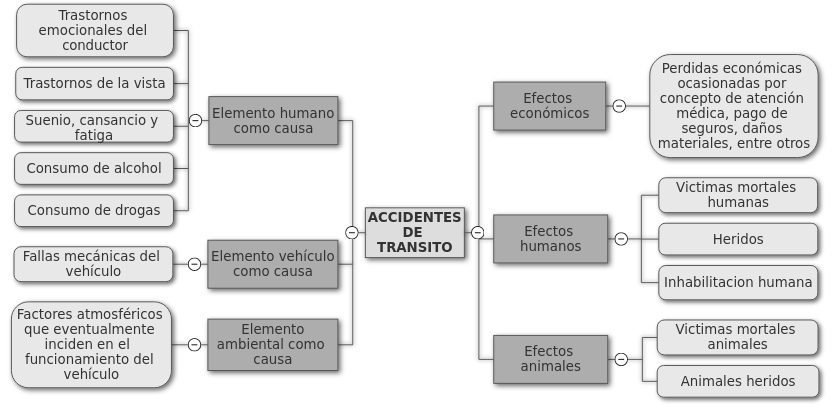
\includegraphics[width=1.0\textwidth]{imagenes/Cap1/arbol_p}
  \caption{\'{A}rbol de problemas}
  \label{fig:arbol}
  \end{center}
\end{figure}

